\documentclass[10pt,a4paper]{article}
\usepackage[margin=2.1cm]{geometry}
\usepackage[T1]{fontenc}
\usepackage{lmodern}
\usepackage{amsmath,amssymb}
\usepackage{booktabs,tabularx,multirow}
\usepackage{enumitem}
\usepackage{xcolor}
\usepackage{tikz}
\usepackage{pgfplots}
\usepackage{caption,subcaption}
\usepackage[hidelinks]{hyperref}
\pgfplotsset{compat=1.18}
\usetikzlibrary{arrows.meta,positioning,fit,backgrounds,calc,shapes.geometric}

\definecolor{ink}{HTML}{1F2A44}
\definecolor{accent}{HTML}{1F4E79}
\definecolor{star}{HTML}{C0392B}
\definecolor{soft}{HTML}{EEF2F7}
\definecolor{mute}{HTML}{8A94A6}
\definecolor{good}{HTML}{2E7D32}
\definecolor{c1}{HTML}{8A94A6}
\definecolor{c2}{HTML}{4F81BD}
\definecolor{c3}{HTML}{C0392B}

\setlist{nosep,leftmargin=*}
\setlength{\parskip}{4pt}
\setlength{\parindent}{0pt}
\captionsetup{font=small,labelfont=bf}

\tikzset{
  box/.style={draw=ink, rounded corners=2pt, fill=white, align=center, font=\footnotesize, minimum height=0.9cm, text width=2.35cm, inner sep=3pt},
  starbox/.style={box, draw=star, line width=0.9pt, fill=star!6},
  llm/.style={box, fill=accent!8, draw=accent},
  arr/.style={-{Stealth[length=2.2mm]}, ink, line width=0.6pt},
  lane/.style={draw=mute, dashed, rounded corners=4pt, inner sep=6pt},
  lanelabel/.style={font=\scriptsize\bfseries, text=mute, anchor=south west},
}

\newcommand{\STAR}{\textsc{STAR}}

\begin{document}

\begin{center}
{\LARGE\bfseries\color{ink} \STAR: Structure-aware Typed Adaptive Retrieval}\\[4pt]
{\large A smart knowledge base for agents over high-stakes financial documents}\\[6pt]
{\small CognitionNext '26 \textbullet\ Problem Statement 1 \textbullet\ Interim technical report (work in progress)}
\end{center}

\vspace{2pt}
\noindent\fcolorbox{accent}{soft}{\begin{minipage}{0.97\linewidth}
\small
\textbf{Summary.} We treat retrieval as \emph{choosing a calibrated evidence set}, not ranking a top-$k$ list.
\STAR\ splits documents into paragraph-sized typed units and builds a catalogue with a \emph{version-family lattice}, so near-duplicate documents become structure rather than noise.
It then scores every candidate paragraph with a learned, query-relative model, propagates evidence over a paragraph graph, and returns the set that maximises expected precision and recall for that particular question.
Selection uses no LLM calls; each query makes exactly one LLM call, to write the answer.
On the training set (all 100 questions, held-out folds, free text-overlap proxy) \STAR\ reaches retrieval F1 $0.31$ against $0.15$ for the banned hybrid-search baseline, and recall $0.67$ against $0.25$.
These are early numbers. Section~\ref{sec:next} lists the known gaps and the next fixes.
\end{minipage}}

\tableofcontents
\vspace{4pt}\hrule

%======================================================================
\section{The problem and how it is scored}

Given a question and an unorganised dump of PDFs, the system must return a grounded answer, the paragraphs it used (with document and page), and a step-by-step trace.
It is scored on four LLM-judged metrics plus cost and latency.
We read the organisers' evaluation notebook closely, because the exact scoring shapes the design.

\begin{table}[h]
\centering\small
\begin{tabularx}{\linewidth}{@{}lX@{}}
\toprule
\textbf{Metric} & \textbf{How the official evaluator computes it (judge: \texttt{deepseek-v4.1-flash}, temperature 0)} \\
\midrule
Answer precision & Both answers are split into atomic points. $1 - \frac{\#\text{our points not supported by gold}}{\#\text{our points}}$ \\
Answer recall & $\frac{\#\text{gold points covered by our answer}}{\#\text{gold points}}$ \\
Context precision & One judge call sees all returned chunks: $\frac{\#\text{judged relevant}}{\#\text{returned}}$ \\
Context recall & $\frac{\#\text{judged relevant}}{\#\textbf{gold chunks}}$. \emph{Count-based and not capped at 1.} \\
\bottomrule
\end{tabularx}
\caption{Scoring definitions from the official notebook.}
\label{tab:metrics}
\end{table}

\textbf{Three consequences drive the whole design.}
\begin{enumerate}
\item \textbf{Granularity is set by the recall denominator.} The median question has 81 gold chunks. Ten big, correct chunks cap recall at about $0.12$, so evidence units must be paragraph-sized and \emph{how many} we return must change per question.
\item \textbf{Any point not in the gold answer lowers precision}, even if it is true. Answers must use only retrieved evidence.
\item \textbf{The judge breaks on long answers} (Section~\ref{sec:judge}), so answers must stay under about 700 words.
\end{enumerate}

%======================================================================
\section{What the training data shows}

\subsection{Corpus and questions}

\begin{table}[h]
\centering\small
\begin{tabular}{@{}lr@{\hspace{2.2em}}lr@{}}
\toprule
\multicolumn{2}{c}{\textbf{Corpus}} & \multicolumn{2}{c}{\textbf{Questions (100)}} \\
\midrule
PDFs & 35 & A: credit analysis of annual reports & 36 \\
Pages (parsed) & 6{,}970 & B: Basel vs US capital proposals & 32 \\
Scanned pages needing OCR & 97 & C: CECL accounting \& quant models & 32 \\
Largest document (distractor) & 1{,}982 pp & Gold documents per question & 0--9 \\
Paragraph units produced & 46{,}304 & Gold chunks per question (median) & 81 \\
\bottomrule
\end{tabular}
\caption{Training set. The 1{,}982-page consolidated Basel Framework is never cited in gold: it is a near-duplicate distractor.}
\end{table}

\begin{figure}[h]
\centering
\begin{subfigure}[t]{0.48\linewidth}
\centering
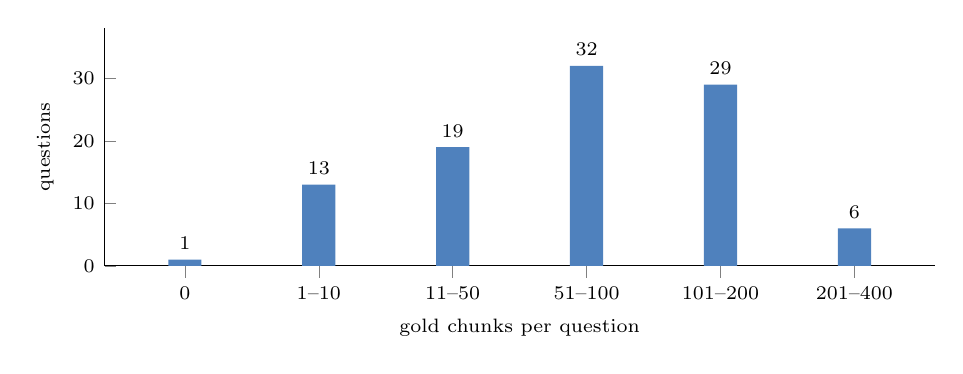
\begin{tikzpicture}
\begin{axis}[ybar, width=\linewidth, height=4.6cm, bar width=12pt,
  symbolic x coords={0,1--10,11--50,51--100,101--200,201--400}, xtick=data,
  x tick label style={font=\scriptsize}, y tick label style={font=\scriptsize},
  ylabel={questions}, ylabel style={font=\scriptsize}, ymin=0, ymax=38,
  nodes near coords, nodes near coords style={font=\scriptsize},
  xlabel={gold chunks per question}, xlabel style={font=\scriptsize}, axis lines*=left, enlarge x limits=0.12]
\addplot[fill=c2, draw=none] coordinates {(0,1) (1--10,13) (11--50,19) (51--100,32) (101--200,29) (201--400,6)};
\end{axis}
\end{tikzpicture}
\caption{Gold evidence size varies by two orders of magnitude, so a fixed $k$ fails in both directions.}
\end{subfigure}\hfill
\begin{subfigure}[t]{0.48\linewidth}
\centering
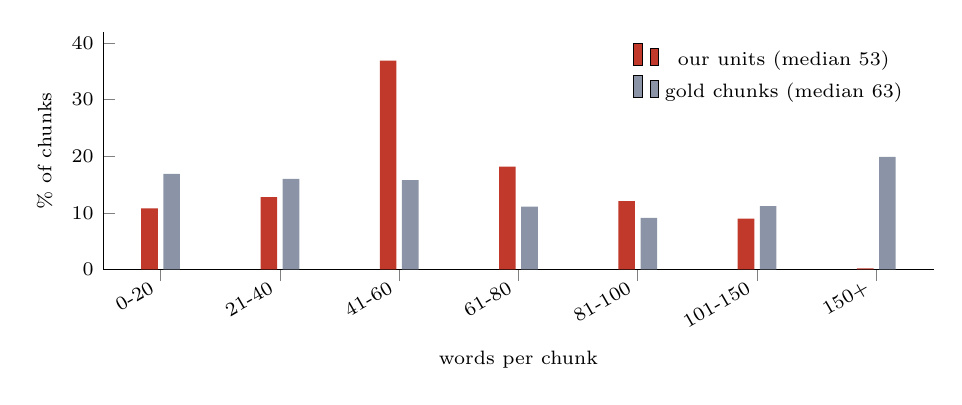
\begin{tikzpicture}
\begin{axis}[ybar, width=\linewidth, height=4.6cm, bar width=6pt,
  symbolic x coords={0-20,21-40,41-60,61-80,81-100,101-150,150+}, xtick=data,
  x tick label style={font=\scriptsize, rotate=30, anchor=east}, y tick label style={font=\scriptsize},
  ylabel={\% of chunks}, ylabel style={font=\scriptsize}, ymin=0, ymax=42, axis lines*=left,
  legend style={font=\scriptsize, draw=none, at={(0.98,0.98)}, anchor=north east}, enlarge x limits=0.08,
  xlabel={words per chunk}, xlabel style={font=\scriptsize}]
\addplot[fill=c3, draw=none] coordinates {(0-20,10.8) (21-40,12.8) (41-60,36.9) (61-80,18.2) (81-100,12.1) (101-150,9.0) (150+,0.2)};
\addplot[fill=c1, draw=none] coordinates {(0-20,16.9) (21-40,16.0) (41-60,15.8) (61-80,11.1) (81-100,9.1) (101-150,11.2) (150+,19.9)};
\legend{our units (median 53), gold chunks (median 63)}
\end{axis}
\end{tikzpicture}
\caption{Our paragraph units are sized like the gold chunks. Gold has a long tail of large tables.}
\end{subfigure}
\caption{Evidence size statistics.}
\end{figure}

The gold chunks were clearly made by a vision-language document parser. Their section names split into prose (4{,}838), markdown tables (1{,}056), LaTeX formulas (277) and image descriptions (68).
So table handling matters a lot, and a small number of facts exist only as images.

\subsection{Relevance clusters along the document}
\label{sec:homophily}

Gold evidence for one question and document spans a median of 9 pages, in about 5 separate runs.
We mapped gold chunks onto our units by word 4-gram overlap and measured \emph{homophily}: how much more likely a unit is to be relevant when its graph neighbour is.

\begin{figure}[h]
\centering
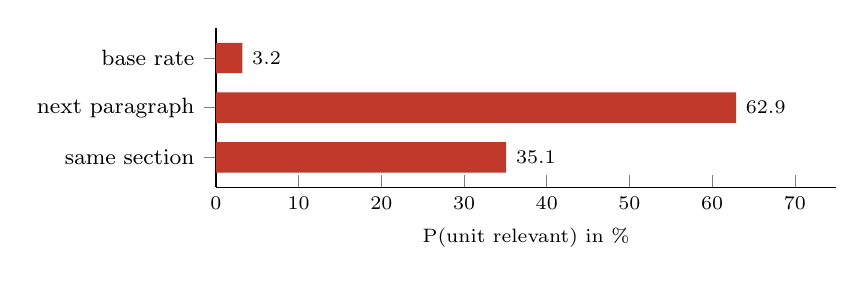
\begin{tikzpicture}
\begin{axis}[xbar, width=0.78\linewidth, height=3.6cm, bar width=11pt,
  symbolic y coords={same section, next paragraph, base rate}, ytick=data,
  y tick label style={font=\footnotesize}, x tick label style={font=\scriptsize},
  xmin=0, xmax=75, xlabel={P(unit relevant) in \%}, xlabel style={font=\scriptsize},
  nodes near coords, nodes near coords style={font=\scriptsize}, axis lines*=left, enlarge y limits=0.3]
\addplot[fill=c3, draw=none] coordinates {(35.1,same section) (62.9,next paragraph) (3.2,base rate)};
\end{axis}
\end{tikzpicture}
\caption{If a paragraph is relevant, the next paragraph is relevant 62.9\% of the time, \textbf{19$\times$ the 3.2\% base rate}. A paragraph in the same section is relevant 11$\times$ as often. This is the empirical case for a graph layer.}
\label{fig:homophily}
\end{figure}

\subsection{The judge's behaviour}
\label{sec:judge}

\begin{figure}[h]
\centering
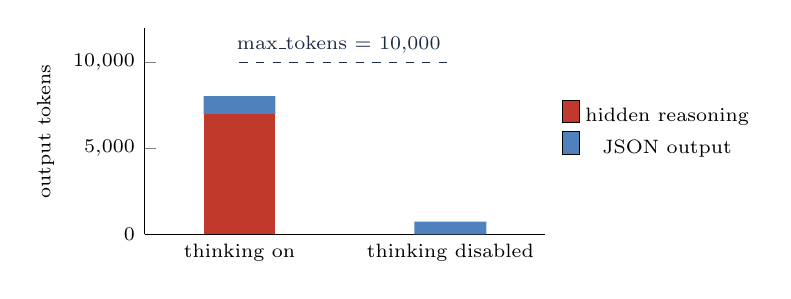
\begin{tikzpicture}
\begin{axis}[ybar stacked, width=0.55\linewidth, height=4.2cm, bar width=26pt,
  symbolic x coords={thinking on, thinking disabled}, xtick=data,
  x tick label style={font=\scriptsize}, y tick label style={font=\scriptsize},
  ylabel={output tokens}, ylabel style={font=\scriptsize}, ymin=0, ymax=12000, axis lines*=left, scaled y ticks=false,
  legend style={font=\scriptsize, draw=none, at={(1.02,0.5)}, anchor=west}, enlarge x limits=0.45]
\addplot[fill=c3, draw=none] coordinates {(thinking on,6980) (thinking disabled,0)};
\addplot[fill=c2, draw=none] coordinates {(thinking on,1071) (thinking disabled,747)};
\draw[dashed, ink] (axis cs:thinking on,10000) -- (axis cs:thinking disabled,10000) node[pos=1, above left, font=\scriptsize] {max\_tokens = 10{,}000};
\legend{hidden reasoning, JSON output}
\end{axis}
\end{tikzpicture}
\caption{Tokens the judge used to split one 654-word gold answer into points. With the notebook's settings, reasoning takes 87\% of the budget. Answers much longer than this exhaust it, the call returns no content, and the question cannot be scored.}
\label{fig:judge}
\end{figure}

\begin{itemize}
\item In our first oracle run (answers written from the gold chunks), answers ran 1{,}000--4{,}600 words and \textbf{the official judge failed on 18 of 24 questions}. \STAR\ therefore caps answers at about 700 words, near the gold median of 754.
\item \textbf{The judge rejects about 25\% of gold chunks} as irrelevant, so returning exactly the gold chunks scores only about $0.75$ on context metrics. The selector should learn \emph{what the judge accepts}, not only what gold contains.
\item One question (A36) is a version trap: it asks about FY2025, but the corpus holds only the 2024 report, and the judge rejected every chunk. Version awareness is enforced by the judge itself.
\end{itemize}

%======================================================================
\section{The \STAR\ architecture}

\STAR\ has six layers. LLM calls happen only once per \emph{document} at ingestion (the catalogue card) and once per \emph{query} (the answer). Everything between runs locally on CPU in milliseconds.

\begin{figure}[h!]
\centering
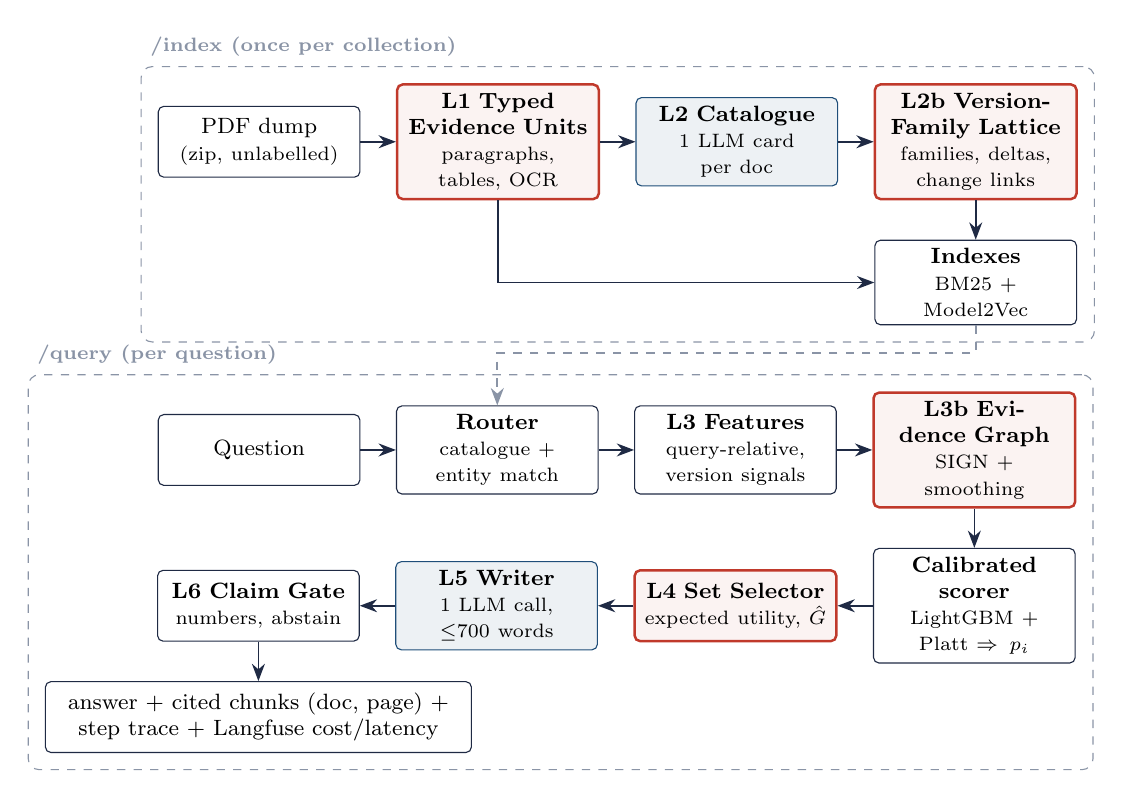
\begin{tikzpicture}[node distance=0.55cm and 0.45cm]
% index lane
\node[box] (pdf) {PDF dump\\\scriptsize(zip, unlabelled)};
\node[starbox, right=of pdf] (teu) {\textbf{L1 Typed Evidence Units}\\\scriptsize paragraphs, tables, OCR};
\node[llm, right=of teu] (cat) {\textbf{L2 Catalogue}\\\scriptsize 1 LLM card per doc};
\node[starbox, right=of cat] (lat) {\textbf{L2b Version-Family Lattice}\\\scriptsize families, deltas, change links};
\node[box, below=0.5cm of lat] (idx) {\textbf{Indexes}\\\scriptsize BM25 + Model2Vec};
\draw[arr] (pdf) -- (teu); \draw[arr] (teu) -- (cat); \draw[arr] (cat) -- (lat); \draw[arr] (lat) -- (idx);
\draw[arr] (teu.south) |- (idx.west);
\begin{scope}[on background layer]
\node[lane, fit=(pdf)(teu)(cat)(lat)(idx)] (lane1) {};
\end{scope}
\node[lanelabel] at (lane1.north west) {/index (once per collection)};

% query lane
\node[box, below=3.0cm of pdf] (q) {Question};
\node[box, right=of q] (route) {\textbf{Router}\\\scriptsize catalogue + entity match};
\node[box, right=of route] (feat) {\textbf{L3 Features}\\\scriptsize query-relative, version signals};
\node[starbox, right=of feat] (graph) {\textbf{L3b Evidence Graph}\\\scriptsize SIGN + smoothing};
\node[box, below=0.5cm of graph] (cal) {\textbf{Calibrated scorer}\\\scriptsize LightGBM + Platt $\Rightarrow p_i$};
\node[starbox, left=of cal] (sel) {\textbf{L4 Set Selector}\\\scriptsize expected utility, $\hat G$};
\node[llm, left=of sel] (write) {\textbf{L5 Writer}\\\scriptsize 1 LLM call, $\le$700 words};
\node[box, left=of write] (gate) {\textbf{L6 Claim Gate}\\\scriptsize numbers, abstain};
\draw[arr] (q) -- (route); \draw[arr] (route) -- (feat); \draw[arr] (feat) -- (graph); \draw[arr] (graph) -- (cal);
\draw[arr] (cal) -- (sel); \draw[arr] (sel) -- (write); \draw[arr] (write) -- (gate);
\node[box, below=0.5cm of gate, text width=5.2cm] (out) {answer + cited chunks (doc, page) + step trace + Langfuse cost/latency};
\draw[arr] (gate) -- (out);
\draw[arr, mute, dashed] (idx.south) -- ++(0,-0.35) -| (route.north);
\begin{scope}[on background layer]
\node[lane, fit=(q)(route)(feat)(graph)(cal)(sel)(write)(gate)(out)] (lane2) {};
\end{scope}
\node[lanelabel] at (lane2.north west) {/query (per question)};
\end{tikzpicture}
\caption{\STAR\ pipeline. Red boxes are our main contributions; blue boxes are the only LLM calls.}
\label{fig:star}
\end{figure}

\subsection*{L1 Typed Evidence Units (fixes the chunk-size dilemma)}
Each page is extracted with PyMuPDF. Pages with no text layer go through Tesseract OCR.
Running headers and footers are removed, and number-heavy pages pass through table detection, so each table becomes one markdown unit.
Prose blocks are merged or split to 40--150 words, with headings tracked as a section path.
\emph{Completeness comes from how many units we select, not from making units bigger.}
The training corpus (6{,}970 pages) ingests in about 6 minutes on a laptop CPU.

\subsection*{L2 Catalogue and L2b Version-Family Lattice (fixes near-duplicates)}
One cheap LLM call per document fills a typed card: title, issuer, entities, document type, jurisdiction, period, date and topics. The 35 cards cost \$0.025 in total.
The lattice then groups documents into version families. It uses text containment between documents ($|A\cap B|/|A|$ over word 5-gram shingles) and joins pairs with union-find.

\begin{figure}[h]
\centering
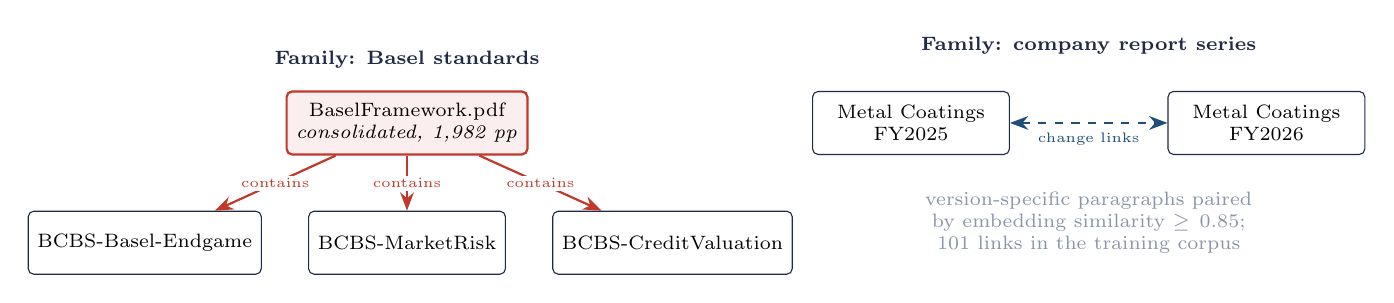
\begin{tikzpicture}[doc/.style={draw=ink, rounded corners=2pt, fill=white, font=\scriptsize, align=center, minimum width=2.5cm, minimum height=0.8cm},
  cons/.style={doc, draw=star, fill=star!8, line width=0.8pt}]
\node[cons] (bf) {BaselFramework.pdf\\\textit{consolidated, 1{,}982 pp}};
\node[doc, below left=0.7cm and 0.3cm of bf] (eg) {BCBS-Basel-Endgame};
\node[doc, below=0.7cm of bf] (mr) {BCBS-MarketRisk};
\node[doc, below right=0.7cm and 0.3cm of bf] (cv) {BCBS-CreditValuation};
\foreach \n in {eg,mr,cv} \draw[-{Stealth}, star, thick] (bf) -- (\n) node[midway, font=\tiny, fill=white, inner sep=1pt] {contains};
\node[doc, right=3.6cm of bf] (m25) {Metal Coatings\\FY2025};
\node[doc, right=2.0cm of m25] (m26) {Metal Coatings\\FY2026};
\draw[{Stealth}-{Stealth}, accent, thick, dashed] (m25) -- (m26) node[midway, below, font=\tiny] {change links};
\node[font=\scriptsize, text=mute, below=0.75cm of $(m25)!0.5!(m26)$, text width=4.6cm, align=center] {version-specific paragraphs paired by embedding similarity $\ge 0.85$; 101 links in the training corpus};
\node[font=\scriptsize\bfseries, text=ink, above=0.15cm of bf] {Family: Basel standards};
\node[font=\scriptsize\bfseries, text=ink, above=0.75cm of $(m25)!0.5!(m26)$] {Family: company report series};
\end{tikzpicture}
\caption{Two of the five version families found automatically. The consolidated Basel Framework, the distractor, is flagged because it contains most of its smaller siblings.}
\label{fig:lattice}
\end{figure}

Each unit is tagged \emph{shared} (its text exists in another version) or \emph{delta}. The training corpus has 4{,}534 shared and 41{,}770 delta units.
Query intent is classified by rules: comparison words, or two or more years, mean \emph{compare}; anything else is \emph{single}.
Intent becomes soft features: ``compare $\times$ has family'' and ``single $\times$ wrong period''.
This follows the idea of VersionRAG \cite{versionrag}, reimplemented in our code, with two differences: it uses no LLM per query, and it detects consolidated texts.

\subsection*{L3 Query-relative features and calibrated scoring}
The router scores documents from card BM25, the top paragraph similarities and entity-name hits, and keeps the top 10 documents as a soft candidate pool.
Every paragraph in the pool gets 25 features: dense and BM25 scores as raw values, z-scores and percentiles \emph{within the pool}; document route score; neighbour and section maxima; table flag; number overlap with the query; and the lattice signals.
Because every feature is relative to the query, the model transfers to a corpus it has never seen.
A LightGBM classifier is trained with 5 folds grouped by question, and Platt scaling turns its scores into probabilities $p_i$.

\subsection*{L3b Evidence Graph (uses the 19$\times$ homophily)}

\begin{figure}[h]
\centering
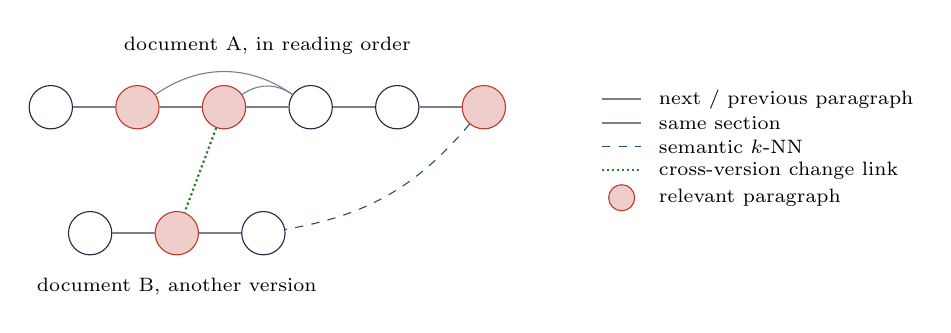
\begin{tikzpicture}[n/.style={circle, draw=ink, minimum size=0.55cm, font=\tiny, fill=white},
  r/.style={n, fill=star!25, draw=star}, e/.style={ink!60}, k/.style={accent, dashed}, c/.style={good, thick, densely dotted}]
\node[n] (a1) at (0,0) {};
\node[r] (a2) at (1.1,0) {};
\node[r] (a3) at (2.2,0) {};
\node[n] (a4) at (3.3,0) {};
\node[n] (a5) at (4.4,0) {};
\node[r] (a6) at (5.5,0) {};
\foreach \x/\y in {a1/a2,a2/a3,a3/a4,a4/a5,a5/a6} \draw[e, thick] (\x) -- (\y);
\draw[e] (a2) to[bend left=35] (a4);
\draw[e] (a3) to[bend left=35] (a4);
\node[n] (b1) at (0.5,-1.6) {};
\node[r] (b2) at (1.6,-1.6) {};
\node[n] (b3) at (2.7,-1.6) {};
\foreach \x/\y in {b1/b2,b2/b3} \draw[e, thick] (\x) -- (\y);
\draw[k] (a6) to[bend left=20] (b3);
\draw[c] (a3) -- (b2);
\node[font=\scriptsize, anchor=south] at (2.75,0.55) {document A, in reading order};
\node[font=\scriptsize, anchor=north] at (1.6,-2.05) {document B, another version};
\begin{scope}[shift={(7.0,-0.2)}]
\draw[e, thick] (0,0.3) -- (0.5,0.3); \node[font=\scriptsize, anchor=west] at (0.6,0.3) {next / previous paragraph};
\draw[e] (0,0) -- (0.5,0); \node[font=\scriptsize, anchor=west] at (0.6,0) {same section};
\draw[k] (0,-0.3) -- (0.5,-0.3); \node[font=\scriptsize, anchor=west] at (0.6,-0.3) {semantic $k$-NN};
\draw[c] (0,-0.6) -- (0.5,-0.6); \node[font=\scriptsize, anchor=west] at (0.6,-0.6) {cross-version change link};
\node[r, minimum size=0.3cm] at (0.25,-0.95) {}; \node[font=\scriptsize, anchor=west] at (0.6,-0.95) {relevant paragraph};
\end{scope}
\end{tikzpicture}
\caption{The evidence graph over one question's candidate pool. Relevant paragraphs come in runs; edges let one strong paragraph lift its weaker neighbours.}
\label{fig:graph}
\end{figure}

We use two graph-learning designs that work with little labelled data, instead of training a deep GNN on 100 questions:
\begin{itemize}
\item \textbf{SIGN / SGC} \cite{sign,sgc}: precompute diffused features $[X,\ \hat A X,\ \hat A^2 X]$ with $\hat A = D^{-1/2}(A+I)D^{-1/2}$, then train LightGBM on them. This is message passing without backpropagation through the graph.
\item \textbf{Correct \& Smooth} \cite{cands}: smooth the predicted probabilities over the graph, $z \leftarrow (1-\alpha)p + \alpha \hat A z$.
\end{itemize}

\subsection*{L4 Expected-Utility Set Selector (decides how much to return)}
Assuming relevance labels are independent given $p_i$, the utility-optimal set is a prefix of units sorted by $p_i$ \cite{ye2012}.
For a prefix of size $k$ with $S_k=\sum_{i\le k}p_{(i)}$ and estimated gold count $\hat G=\sum_i p_i$:
\[
\mathbb{E}[\text{precision}_k]\approx \frac{S_k}{k}, \qquad \mathbb{E}[\text{recall}_k]\approx \min\!\left(1,\ \frac{S_k}{\hat G}\right), \qquad k^\star=\arg\max_k \ \mathrm{F1}\big(\mathbb{E}[P_k],\mathbb{E}[R_k]\big).
\]
A factual lookup gets a handful of units, and a full credit review gets hundreds.
Capping recall at 1 means the objective never rewards splitting text into fragments to inflate the count.

\subsection*{L5 Writer and L6 Claim Gate}
One \texttt{deepseek-v4.1-flash} call with thinking disabled writes the answer from the selected units, in document order and in the gold answers' analyst style (cited \texttt{[file pN]}), using no outside knowledge, in at most about 700 words.
The gate then checks that every number and entity appears in a cited unit, and returns the exact abstention string when even the best $p_i$ is low.

%======================================================================
\section{Comparison architectures}

\begin{table}[h]
\centering\small
\begin{tabularx}{\linewidth}{@{}lXll@{}}
\toprule
\textbf{Row} & \textbf{Design} & \textbf{LLM calls / query} & \textbf{Status} \\
\midrule
\textbf{\STAR} & This report: typed units, lattice, calibrated graph scorer, expected-utility set & 1 (writer) & measured (proxy) \\
1 & Banned baseline: hybrid dense + BM25 (reciprocal rank fusion), fixed top-$k$ & 1 & measured (proxy) \\
2 & LLM-Navigator after the Enterprise RAG Challenge winner \cite{ricerag}: the LLM reads shortlisted pages and picks paragraphs & 1 + pages/6 & built, not run \\
3 & Brute-force long context: the routed documents in one prompt (the PS author's upper bound) & 1 (very long) & planned \\
\bottomrule
\end{tabularx}
\caption{Architectures compared. Rows 2 and 3 anchor the expensive end of the cost-versus-accuracy chart.}
\end{table}

%======================================================================
\section{Results so far}

All retrieval numbers use the \textbf{free text-overlap proxy}: a selected unit counts as correct if most of its word 4-grams appear in a gold chunk, and recall divides by the gold-chunk count, as the official metric does.
They come from all 100 questions, with every learned model evaluated out-of-fold (5 folds grouped by question).

\begin{figure}[h]
\centering
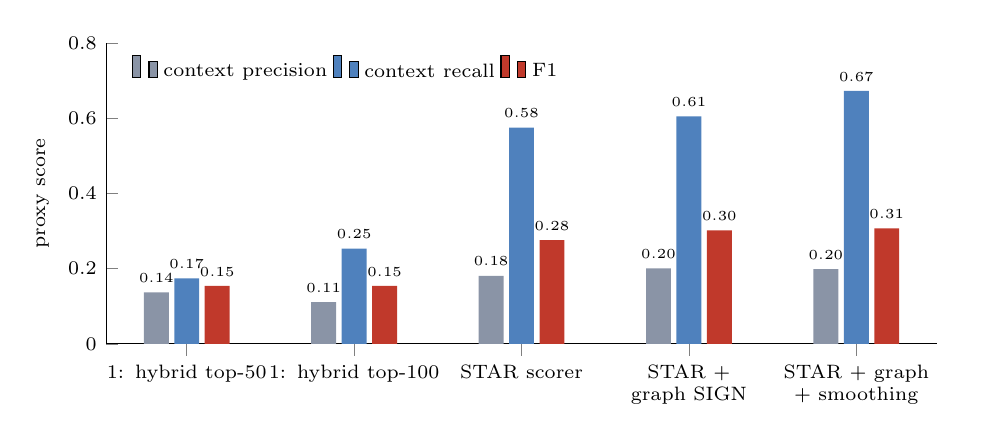
\begin{tikzpicture}
\begin{axis}[ybar, width=\linewidth, height=5.4cm, bar width=9pt,
  symbolic x coords={1: hybrid top-50, 1: hybrid top-100, STAR scorer, STAR + graph SIGN, STAR + graph + smoothing},
  xtick=data, x tick label style={font=\scriptsize, text width=2.3cm, align=center}, y tick label style={font=\scriptsize},
  ymin=0, ymax=0.8, ylabel={proxy score}, ylabel style={font=\scriptsize}, axis lines*=left,
  nodes near coords, nodes near coords style={font=\tiny, /pgf/number format/fixed, /pgf/number format/fixed zerofill, /pgf/number format/precision=2},
  legend style={font=\scriptsize, draw=none, at={(0.02,0.98)}, anchor=north west, legend columns=3}, enlarge x limits=0.12]
\addplot[fill=c1, draw=none] coordinates {(1: hybrid top-50,0.137) (1: hybrid top-100,0.111) (STAR scorer,0.181) (STAR + graph SIGN,0.201) (STAR + graph + smoothing,0.199)};
\addplot[fill=c2, draw=none] coordinates {(1: hybrid top-50,0.174) (1: hybrid top-100,0.253) (STAR scorer,0.575) (STAR + graph SIGN,0.605) (STAR + graph + smoothing,0.673)};
\addplot[fill=c3, draw=none] coordinates {(1: hybrid top-50,0.154) (1: hybrid top-100,0.154) (STAR scorer,0.276) (STAR + graph SIGN,0.302) (STAR + graph + smoothing,0.307)};
\legend{context precision, context recall, F1}
\end{axis}
\end{tikzpicture}
\caption{Retrieval quality on the proxy. \STAR's set selection more than doubles recall over fixed top-$k$, and the graph layer adds recall on top.}
\label{fig:results}
\end{figure}

\begin{table}[h]
\centering\small
\begin{tabular}{@{}lccccc@{}}
\toprule
\textbf{Configuration} & \textbf{P} & \textbf{R} & \textbf{F1} & \textbf{median $k$} & $\rho(\hat G, |\text{gold}|)$ \\
\midrule
1: hybrid RRF, top-20 & 0.177 & 0.097 & 0.126 & 20 & -- \\
1: hybrid RRF, top-100 & 0.111 & 0.253 & 0.154 & 100 & -- \\
LightGBM scores, fixed top-100 & 0.196 & 0.386 & 0.260 & 100 & -- \\
\STAR\ scorer + set selector & 0.181 & 0.575 & 0.276 & 186 & 0.27 \\
\quad + evidence graph (SIGN) & \textbf{0.201} & 0.605 & 0.302 & 172 & 0.31 \\
\quad + Correct \& Smooth ($\alpha=0.5$) & 0.199 & \textbf{0.673} & \textbf{0.307} & 207 & 0.31 \\
\quad ablation: smoothing without SIGN & 0.180 & 0.656 & 0.282 & 200 & 0.27 \\
\bottomrule
\end{tabular}
\caption{Ablation. Each graph component adds measurable recall; SIGN features also add precision.}
\label{tab:ablation}
\end{table}

\paragraph{Routing.} 93.8\% of gold documents land in the candidate pool, and 87.7\% of the gold count is reachable inside it. That is the retrieval ceiling for the current router.

\paragraph{Cost so far.} The whole development run, including judge calls, has spent \$2.11 of the \$10 credit, most of it on judge calls that failed for the reason shown in Figure~\ref{fig:judge}.
\STAR's query path runs no LLM calls until the writer.

%======================================================================
\section{Known gaps and next steps}
\label{sec:next}

\begin{enumerate}
\item \textbf{Proxy precision understates the real score.} The proxy only credits paragraphs that contain gold text, while the judge also accepts relevant paragraphs outside gold (and rejects 25\% of gold). Next: run the judge's relevance check on \STAR's selections for the 24-question subset (about \$0.30) to calibrate proxy against judge.
\item \textbf{The set-size estimate $\hat G$ is weak} (correlation 0.31 with the true gold count), so \STAR\ over-selects (median 172--207 units). Next: a small count model from query features, which directly raises precision.
\item \textbf{Sharper relevance:} add a CPU cross-encoder score on the top few hundred candidates as an extra feature (confirmed allowed), and tighten the 10-document pool.
\item \textbf{Run rows 2 and 3} on the subset to anchor the cost-versus-accuracy chart.
\item \textbf{End-to-end answers:} run the writer on \STAR's selections and score them with the official judge; serve \texttt{/index} and \texttt{/query} with the trace and Langfuse; export the knowledge base as an Open Knowledge Format bundle.
\end{enumerate}

%======================================================================
\begin{thebibliography}{9}\small
\bibitem{versionrag} D.~Huwiler et al. \emph{VersionRAG: Version-aware retrieval-augmented generation.} arXiv:2510.08109, 2025.
\bibitem{sign} E.~Rossi et al. \emph{SIGN: Scalable Inception Graph Neural Networks.} arXiv:2004.11198, 2020.
\bibitem{sgc} F.~Wu et al. \emph{Simplifying Graph Convolutional Networks.} ICML 2019.
\bibitem{cands} Q.~Huang et al. \emph{Combining Label Propagation and Simple Models Out-performs Graph Neural Networks.} ICLR 2021.
\bibitem{ye2012} N.~Ye, K.~Chai, W.~Lee, H.~Chieu. \emph{Optimizing F-measures: A Tale of Two Approaches.} ICML 2012.
\bibitem{ricerag} I.~Rice. \emph{RAG-Challenge-2}, winner of the Enterprise RAG Challenge round 2. github.com/IlyaRice/RAG-Challenge-2 (MIT), 2025.
\end{thebibliography}

\end{document}
